\section{V2X}
    V2X(Vehicle to Everything)은 차량과 다른 모든 대상이 이동통신망을 통해 유기적으로 상호 통신하며 정보를 교환하는 기술이다. 구체적으로 V2V(Vehicle to Vehicle), V2I(Vehicle to Infrastructure), V2N(Vehicle to Nomadic Device), V2P(Vehicle to Pedestrian) 등의 기술을 융합한 것이다. 이러한 V2X 기술은 미래 모빌리티 산업의 핵심으로 주목 받는 커텍티드 카 및 자율주행 기술로 구현되고 있다. 앞서 다룬 VANET 역시 V2X를 활용한 기술이다. \\
    \vspace{-4mm}
    \begin{figure}[!h]\centering
		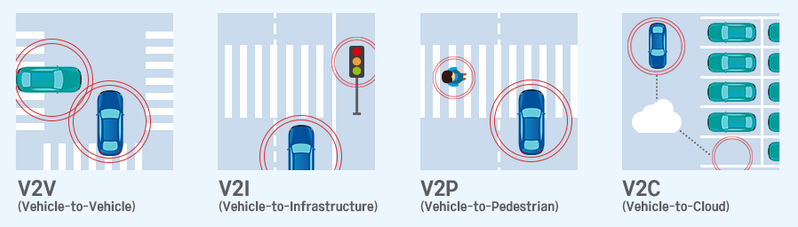
\includegraphics[width=.9\textwidth]{image/week13/3-1.png}
		\caption{\small V2X 구성요소}
		\vspace{-10pt}
    \end{figure}
    
    대표적인 V2X 통신 기술에는 DRSC/WAVE와 C-V2X가 있다. \\
    DRSC/WAVE는 차량과 노변기지국 간 통신을 가능하게 하는 DSRC(Dedicated Short Range Communication)와 고속주행하는 차량에서의 통신을 제공하는 WAVE(Wireless Access in Vehicular Environment) 기술의 조합이다. 2010년 IEEE 802.11a 무선랜(WiFi) 기술을 기반으로 자동차 주행 환경에 적합하도록 IEEE 802.11p로 표준화 되었고, 2016년에는 네트워크 및 전송 계층 표준으로 IEEE 1609.3, 다중접속을 위한 채널할당 표준으로 IEEE 1609.4, 보안 통신 표준으로는 IEEE 1609.2를 개발하였으며 미국자동차공학회(SAE)에서는 V2V 및 V2I간 정보 교환을 위한 메시지 형식을 정의한 J2735 표준과 안전 통신을 위한 단말기 최소 성능 요구사항을 정의한 J2945/1 표준을 개발하였다. WAVE 기술은 지난 10년간 국내외에서 ITS를 비롯한 다양한 첨단 교통 서비스에 사용되어 왔다. \\
    2018년에는 기존 WAVE 기술과 호환성을 유지하면서 통신 성능을 개선하기 위한 NGV(Next Generation V2X, 802.11bd) 표준화 작업이 시작되었다. NGV 표준에서는 채널 복잡도, 가시·비가시 환경 등 다양한 통신 환경을 고려하기 위한 채널 모델을 제안하고 그러한 환경에서 통신 성능을 보장하기 위한 기술들을 논의하고 있다. \\
    C-V2X는 3GPP 이동통신을 기반으로 특정 차량이 다른 차량이나 인프라와 통신하게 해주는 기술이다. C-V2X는 각각 LTE와 5G를 사용하는 LTE-V2X와 5G-V2X로 구분된다. 2017년에 표준을 완료한 LTE-V2X는 WAVE와 유사한 성능과 서비스 제공이 가능할 것으로 예상된다. 2020년에 표준을 완료한 5G-V2X는 높은 신뢰성, 저지연, 고속의 5G 기술을 사용하기 때문에 상용화시 자율주행차의 원격운전, 고밀도 군집주행, 센서정보 공유과 같은 고도의 서비스를 이용할 수 있을 것으로 예상된다. \\
    5G-V2X는 성능에 있어 좋은 평가를 받고 있지만 2026년 상용화를 목표로 하고 있기 때문에 2022년 현재 상용화 사례를 찾기 어렵다. 반면에 WAVE는 10년간 상용화 과정을 거쳐 편의성과 안정성이 검증되었기 때문에 새로운 5G-V2X를 도입하는데 어려움이 있는 상황이다. \\
    \vspace{-4mm}
    \begin{figure}[!h]\centering
		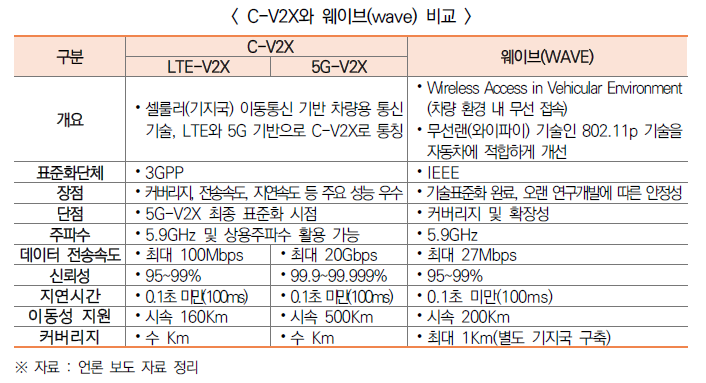
\includegraphics[width=.85\textwidth]{image/week13/3-2.png}
		\caption{\small C-V2X와 WAVE 비교}
		\vspace{-10pt}
    \end{figure}
    
    미국 연방통신위원회(FCC)가 2020년 10월 ‘5.9GHz 현대화’ 규칙 제정안을 공고했다. 5.9GHz 대역을 WiFi와 C-V2X에 할당하고, 기존에 이 대역을 이용하던 WAVE를 2년 내에 C-V2X로 대체한다는 내용이다. 기존의 WAVE 방식으로 C-ITS를 광범위하게 구현하기에는 확장성이 부족하기 때문에 C-V2X를 단일 표준으로 지정한 것으로 분석된다. \\
    유럽위원회는 2006년부터 C-ITS 구축을 위한 계획을 발표하고 준비했다. 2019년 DSRC/WAVE로 C-ITS를 구축하려는 지침을 법제화하는 안을 발의 했으나 부결되었다. 유럽은 기술 중립성을 이유로 단일 표준을 사용하지 않는다. \\
\clearpage